\documentclass[12pt]{article}

\usepackage{url}
\usepackage{cite}
\usepackage[acronym,xindy,toc]{glossaries}
\usepackage{graphicx}
\usepackage{float}
\graphicspath{ {./images/} }

\linespread{1.1}

\makeglossaries

\begin{document}
\title{COEN 332: Web 2.0}
\author{Giovanni Briggs}

\maketitle

\clearpage

\tableofcontents
\clearpage

\phantomsection
\addcontentsline{toc}{section}{List of Figures}
\listoffigures

%Term definitions
\newacronym{qos1}{QoS}{Quality of Service}
\newacronym{tcp}{TCP}{Transport Control Protocol}
\newacronym{ftp}{FTP}{File Transport Protocol}
\newacronym{api}{API}{Application Programmer Interface}
\newacronym{ui}{UI}{User Interface}
\newacronym{rts}{RTS}{Real Time Strategy}
\newacronym{html}{HTML}{HyperText Markup Language}
\newacronym{rdf}{RDF}{Resource Description Framework}
\newacronym{uri}{URI}{Uniform Resource Identifiers}
\newacronym{http}{HTTP}{HyperText Transfer Protocol}
\newacronym{rdfs}{RDFS}{RDF Vocabulary Definition Language}
\newacronym{owl}{OWL}{Web Ontology Language}
\newacronym{xml}{XML}{Extensible Markup Language}
\newacronym{sms}{SMS}{Short Message Service}

%Print the glossary
\glsaddall
\printglossary[type=\acronymtype, nonumberlist] % prints just the list of acronyms
\clearpage

\section{Audience}
This document aims to explain what Web 2.0 is and how it has transformed the way content is created and shared on the Internet.  Much of this discussion will center around comparing Web 2.0 to the an older state of the web, often referred to as Web 1.0.  This document will also explore the concept of the "Liquid Web" which is a natural extension of Web 2.0.  We will dive into how the Liquid Web has transformed the way we interact with applications on the Web.  Finally, we will examine the next evolution of the web to Web 3.0, the "Semantic Web."

This document is for individuals who have some knowledge of how the Internet works but wish to know more about the current state of the World Wide Web and how many people imagine its evolution.  We will examine Web 1.0 in enough detail that even a very basic understanding will be enough.  This document is very light in technical details and instead chooses to focus on very small changes in the way we conceptualize the structure of the web have led to huge improvements in our ability to share, access and create content.

\section{Introduction}
Web 2.0 is the brainchild of Tim O'Reily and was his attempt to explain why certain companies survived the dot-com bubble burst in 2001.  According to O'Reilly, Web 2.0 is really the idea of the "web as a platform." \cite{what_is_web2}.  It is not the servers and the physical pipeline that people are interested in anymore.  In Web 2.0, people are interested in the services provided on top of the Internet.

O'Reily produced this theory in 2005 and it has maintained its popularity in describing how the most successful technology companies today have maintained their online presence.  O'Reily's pinnacle example of the difference between Web 1.0 and Web 2.0 is the comparison between Netscape and Google.  Netscape was the world's first mover in the Internet browser market \cite{netscape_history}.  Netscape then used their popularity and built a host of plugins.  These plugins focused both on useful applications, such as enabling File Transport Protocol (FTP) and enabling better multimedia processing in the browser itself, such as Shockwave.

What killed Netscape in the end was its competition with Microsoft.  Microsoft's Internet Explorer browser which was launched as a free service as part of the Windows operating system.  Netscape couldn't compete with this free and widely distributed piece of software and so they quickly lost their market share, and eventually went out of business \cite{netscape_history}.

Now compare that to Google, which O'Reily hails as the pinnacle of Web 2.0.  Google didn't start by distributing software.  Instead it released a native web application and as such, Google wasn't bound to the same rules of software distribution and management as Netscape.  They can apply updates and changes and it requires no work on the user's end to gain these benefits \cite{what_is_web2}.  Even the competition that Google had with Yahoo!,and other search engines, was different than the competition between Netscape and Microsoft.  Google and Yahoo! could not beat each other simply by making their services cheaper than the other, since both engines are free to use.  They have to focus on the services that they provide and they are able to release and distribute those faster than a traditional, Web 1.0 company could.  Ironically, these search engines would not have become popular without the web browser which allowed users to find and access the engines in the first place.

This leads to O'Reily's four main principles of Web 2.0 \cite{what_is_web2}:
\begin{enumerate}
  \item{The value of the software is proportional to the scale and dynamism of the data it helps to manage}
  \item{Leverage customer-self service and algorithmic data management to reach out to the entire web, to the edges and not just the center, to the long tail and not just the head}
  \item{The service automatically gets better the more people use it}
  \item{Network effects from user contributions are the key to market dominance in the Web 2.0 era}
\end{enumerate}

What O'Reily argued in 2005 was that the web needed to be more open-sourced.  The power of the Web should not remain in the hands of a few corporations, but rather, should be harnessed from the contributions and experiences of its daily users.  O'Reily mentions Sourceforge multiple times as an example of the power of open source contributions.  The web as a platform model should enable everyone to make contributions, and gain from the contributions of others.  Today, we can see that O'Reily's predictions about open-source were correct.  Google's Chrome browser allows for user developed plugins.  GitHub, which was founded in 2008, has become the most popular way for distributing and managing open source projects.  Even package managers such as "pip" for Python and "npm" for Node.JS enable developers to access and leverage the work of other developers.

O'Reily also spends a great deal of time discussing that user data is the main commodity for Web 2.0 companies \cite{what_is_web2}.  We see this in Google's revenue structure.  The majority of their revenue comes from delivering targeted advertisements to its users.  That targeting requires them to collect data on their users and so that data becomes their primary commodity \cite{google_revenue}.  This trend is also seen in Facebook, Twitter, and really all of the social media sites make money.  They do not sell a software, but instead, sell data.  In the new age of Web 2.0, if you are not paying from the product, then you are the product\cite{social_media_revenue}.

Another benefit to the Web 2.0 design is that users are no longer tied to a single device \cite{what_is_web2}.  Since the Internet can be accessed by pretty much everything these days, a user should be able to access their information from anywhere and have a rather seamless experience.  Today, we see this in Google's architecture.  With one Google account, I can access my information from my desktop, my phone, and even other computers whenever I want.  Gaming has also made significant strides in this area of having a fluid experience.  Sony and Microsoft both offer their users the ability to play a game on their flagship console, while also allowing the user to then pick up that same game experience on another device.  For Microsoft more specifically, a user can begin playing a game on their XBox One, and then pick up right where they left off on their laptop.  Sony goes one step further and allows users to continue playing on a dedicated mobile device so that users can play anywhere they want.

In today's world, Web 2.0 has very much become the standard, but the remnants of Web 1.0 are not gone completely.  To understand the Web's current state and its future, we need to take a step back and look at the process that started all of it.  Section 3 will examine the key characteristics of Web 1.0 and how it evolved into Web 2.0.  This discussion will include the archtiecture of Web 2.0  adn how that archtiecture has changed the way people share and access content.  We will also take some time to discuss the criticism of Web 2.0 and why some people don't believe it is a real concept.  Section 4 will dive into the "Liquid Web" which is natural extension of Web 2.0 which allows users to seamlessly transition their experiences between different devices through web connectivity.  Section 4 will also examine how the Liquid Web is not just more convenient for users, but also how it transforms our interactions with media content such as videos and video games. In Section 5, we will look at the next step of web evolution to the "Semantic Web", also referred to as "Web 3.0" and how it uses Web 2.0 and Web 1.0 as its main backbone.

\section{Web 1.0 vs Web 2.0}
In order to better understand what Web 2.0 is, it is important to identify the key characteristics of Web 1.0.  It is also important to keep in mind that Web 1.0 and Web 2.0 is not trying to identify different versions of the web in the same way that we say that \textit{software package version 1} is different than \textit{software package version 2}.  Instead Web 1.0 and Web 2.0 refer to paradigm shifts in the way that we create, share and model our websites.

The major difference between Web 1.0 and Web 2.0 is that in Web 1.0, users were simply consumers of content and information.  In Web 2.0, any user can be a creator of content \cite{FM2125}.  Again, the idea of Web 2.0 is that it is the web as a platform.  Everyone is able to contribute content to a website.  This includes creating and hosting their own blogs and tagging already published content.

\begin{figure}[H]
  \begin{center}
    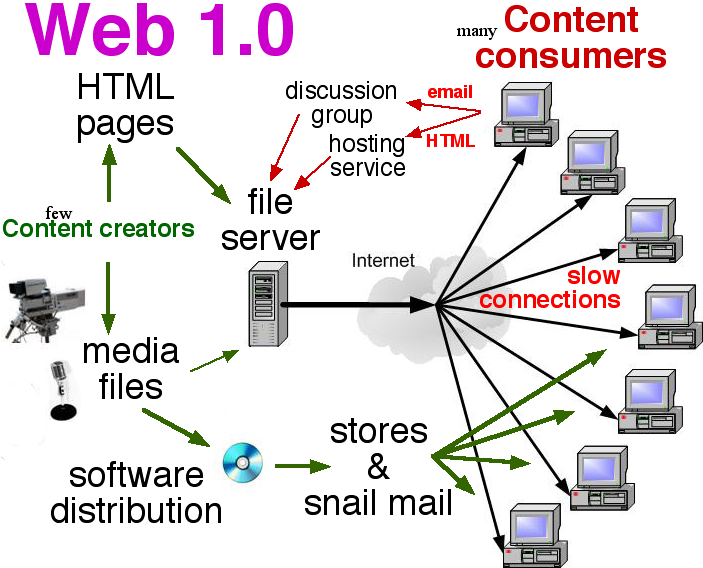
\includegraphics[scale=0.4]{Web_1.0_elements.png}
    \caption{Elements of a Web 1.0 website}
    \label{fig:web1elements}
  \end{center}
\end{figure}

For Web 1.0, website content was static.  As Figure \ref{fig:web1elements} shows, there were many content consumers, but there were very few content consumers.  Consumers accessed HTML web pages by connecting to the file server, and that single server was responsible for serving that data to every user that requested it.  Email threads and mailing lists were the primary form of communicating with other people on the web.  Compared to today's instant messaging, mailing lists are not nearly as instantaneous or fluid.  Many mailing lists today also do not support everyone asking questions.  A few people have the ability to send relevant content out to the list, but not everyone can add content into the thread.  This is yet another example of a Web 1.0 technology vs a Web 2.0 technology.  Instant messaging lets a group of people chat at the same time.  Every user can be a content creator vs email mailing lists in which there could be many consumers, but only a few content creators.

Web 1.0 can be further broken down by the following characteristics \cite{is_there_web_1}:

\begin{enumerate}
  \item {Web 1.0 sites are static.  Web 2.0 sites then are \textit{dynamic}}
  \item {Web 1.0 sites aren't interactive. Web 2.0 sites then \textit{are} interactive.}
  \item {Web 1.0 applications are proprietary.  Web 2.0 then are either \textit{open sourced} or have open \textit{Application Programmer Interfaces}e (API).}
\end{enumerate}

Web 1.0 sites are not dynamic or interactive and these applications are proprietary.  Once again, the theme here is that Web 1.0 revolves around a few content creators and many content consumers.  By contrast then, Web 2.0 is a more open web in which all of the users have the ability to become a contributor and a developer.

\subsection{Determining Web 1.0 vs Web 2.0}
Defining one website as Web 1.0 or Web 2.0 is difficult.  In part because the underlying technology that powers them is the same.  Generally speaking though Web2.0 sites can be identified by the following characteristics \cite{FM2125}:
\begin{enumerate}
  \item{the use of AJAX or other technologies that enable Web pages to load content dynamically}
  \item{Web sites which incorporate a strong social component, involving user profiles, friend links}
  \item{Web sites which encourage user–generated content in the form of text, video, and photo postings along with comments, tags, and ratings}
\end{enumerate}

Most social media sites, which were really beginning to grow rapidly in the earl 2000s, qualify as Web 2.0.  Within Facebook for example, users are the main content providers.  Most of what you see on a Facebook page is status updates and photos from the people you've connected with.  There is also professionally published content from news sites and other sources, but every user has the ability to directly contribute content.

\begin{figure}[H]
  \begin{center}
    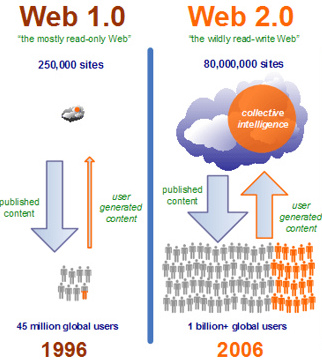
\includegraphics[scale=0.8]{web3_3.jpg}
    \caption{Comparison between Web 1.0 and Web 2.0}
    \label{fig:web3_3}
  \end{center}
\end{figure}

Figure \ref{fig:web3_3} gives a quick look at this difference.  In Web 2.0 there is more user generated content.  The Web is now not just a read only medium, but also gives the average user the ability to leave their mark.  The ability of user's to write content isn't the only thing that is changing in Web 2.0.  The level of interactivity and dynamism that Web 2.0 requires necessitates different technologies and architectures.

\subsection{Web 2.0 Architecture}
The architecture of a Web2.0 site needs to be different than a Web 1.0 site.  In Web 1.0, sites simply had content.  When a user wanted the content, the site would serve it to them. In Web 2.0, we now have users contributing data, but we also need people to be able to receive the updates that new content has been published.

Figure \ref{fig:web2_arch} shows this publish and subscribe architecture.  This figure shows some of the different ways in which some users \textit{publish}  content and how that content makes its way onto consumers's \textit{displays} \cite{FM2125}.  There are are also two different types of content, and two different ways to send that data to consumers.  First, micro-content is smaller, quick content such as a Facebook status update or a Twitter "tweet."  This content is often created quickly and therefore there is a lot more of it.  Macro-content is user created content that takes a longer time to consume.  A blog post is significantly larger than a 140-character tweet. A YouTube video is not only time consuming to view, but is also simply very large in terms of its file size.  There is also a spectrum of ways to push that content to consumers, ranging from more intrusive forms of updates such as the Short Messaging Service (SMS), and less intrusive forms such as keeping Facebook status update within the Facebook app \cite{FM2125}.

\begin{figure}[H]
  \begin{center}
    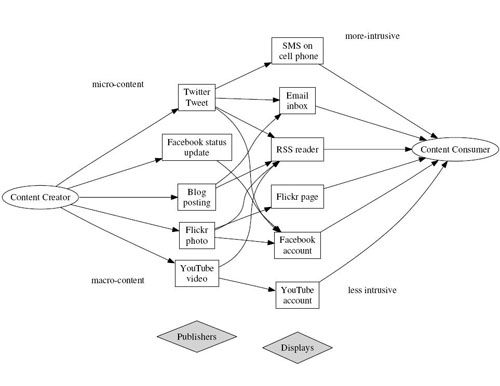
\includegraphics[scale=0.8]{web2_arch.jpg}
    \caption{Web 2.0 publish and subscribe architecture.}
    \label{fig:web2_arch}
  \end{center}
\end{figure}

The reason that SMS is more "intrusive" is because it happens immediately and hits the user on their mobile device.  The user doesn't necessarily have the ability to avoid the update.  They are always connected and in touch with these updates.  Keeping notifications contained within the site, such as a Facebook status update that only shows up within Facebook, is less intrusive because the user is in control of when they want to view the content.  The user can chose to login to Facebook and view the status updates when they are ready.

The article that we have been referencing in throughout this document was written in 2008, and much has changed in what a user considers "intrusive" and "not intrusive."  While SMS is still a way for content providers to send their updates to consumers, most updates now seem to happen through notifications that occur natively on a consumer's smartphone.  With a dedicated mobile app, an application can push content and updates directly to the users device, without the need of SMS.  This has become so commonplace today that many users may no longer feel like this type of notification is "intrusive", rather, it has become expected.

The ability to manually push content to these sites comes with a natural progression - automation.  While any user can now generate content and share it with the world, major publishers still have a major stake in using the same channels, but these publishers are already publishing their static content to their own sites.  Publishers want to be able to write their content but then have it shared out on other sites without friction.

This leads to the creation of Application Programmer Interfaces (API) and they are a defining mark of a Web2.0 site.  These APIs provide developers with the opportunity to interact with the site and do all of the actions a normal user would do, but through a program instead of manual human interaction.  It is also one of the ways in which Web2.0 sites allow every user the opportunity to also be a developer.  Anyone with the correct credentials (and they are typically not hard to get) can interact with the site.  This can be used to push more content to the site, or to provide secondary value by accessing the data the site contains.  For example, Facebook's API has given rise to many apps that send content to Facebook on behalf of the user and also apps that analyze a user's patterns on Facebook.

Again, the major difference between this and Web 1.0 is that the technologies that power Web 2.0 sites are made public through the use of APIs.  This also helps enable every user to be a content creator instead of just a content consumer.

\subsection{Publishing Content on Web 2.0}
As we've mentioned, the hallmark of Web 2.0 is the ability for anyone to create content and share it on the web.  It helps to understand in more detail how this increase in content has shaped how we handle it.

Bryan Alexander and Alan Levin argue that Web 2.0 has changed the way that people tell stories on the web.  There are two essential features: microcontent and social media \cite{web_2_storytelling}.

Microcontent, which we have discussed earlier in this paper, is the generation of small chunks of content, where each chunk is a contained concept.  For example, these chunks could be blog posts, YouTube comments, or Instagram posts.  The process of uploading them is extremely simply from the user perspective, and the storage of each piece of content is rather small.  But small storage is not the defining property of microcontent.  YouTube videos, which are not small by any means, are also microcontent.  YouTube videos are typically short in nature, and each tries to convey a contained thought.  The outcome of this shift from a handful of publishers creating large, controlled content to many users publishing microcontent is that the friction for participation and publishing is drastically lower.  With more content out there, the competition increases, and consumers can focus more on finding the best content out there \cite{web_2_storytelling}.

The second feature is social media.  Web 2.0 platforms are more structured around users rather than machines and directory trees.  Once you have people creating microcontent, you then need to figure out how to get them to share it, and that necessitates the ability to build a social graph and share your content within that graph \cite{web_2_storytelling}.  Being social and person oriented also allows the data to become more enriched.  User A creates a YouTube video about the upcoming election.  User B comments on the video and leaves a link to a blog post with a different viewpoint.  User C then sends a counter argument.  Now, a consumer not only benefits from User A's original content creation, but also from the discussion that users have centered around that content.  Although for anyone that has ever taken the time to read the comments section, you know that it is rarely this civil.  By giving people the ability to create microcontent whenever they want, you also have to accept the fact that there is going to be a lot of bad content.

\begin{figure}[H]
  \begin{center}
    \includegraphics[scale=0.4]{web_2_storytelling.pdf}
    \caption{Web 2.0 content encompasses a wide range of mediums.}
    \label{fig:web_2_storytelling}
  \end{center}
\end{figure}

Figure \ref{fig:web_2_storytelling} shows the wide range of content that Web 2.0 encompases \cite{web_2_storytelling}.  This figure looks similar to Figure \ref{fig:web2_arch}, but Figure \ref{fig:web_2_storytelling} shows this in terms of the different mediums that Web 2.0 encompasses.  The green boxes are the traditional mediums of Web 1.0 content.  Web 1.0 was still a digital form of content distribution, but it didn't have the same scale as Web 2.0.  Web 2.0 includes oral storytelling through the form of videos and podcasts on platforms such as YouTube and even iTunes.  Since Web 2.0 also drastically reduced the cost of publication, it put traditional publishers, like newspapers, in a hard spot.  It required them to start moving their content to the web as well (although whether or not traditional newspapers can be saved is a different discussion) \cite{kennedy_2016}.

Again, the point of Web 2.0 is that by decreasing the friction in publishing content, it allowed anyone to share their content on the web.  This shift though necessitated several other features, namely, a more user-centric architecture.

\subsection{Criticism of Web 2.0}
Not everyone agrees the Web 2.0 is a real shift in the way that people use the Web.  Web founder Tim Berners-Lee, is the chief critic, claiming that Web 2.0 isn't very well defined at all and isn't any different than "Web 1.0." \cite{web_2_criticism}.

Berners-Lee argues that the Web 2.0 doctrine claims that Web 2.0 is about connecting people to people, not just people to content; however, connecting people to other people was what the Web was designed for in the first place.  Berners-Lee also points out that while Web 2.0 has a set of "standards," it struggles to find the common characteristics that make one site Web 2.0 and another site Web 1.0.  Even in this paper, the examples listed can feel contrived.  For Berners-Lee, Web 2.0 is just a fancy catchphrase that people are using but that has no real substance to it.  Some people went even further than Berners-Lee and began comparing Web 2.0 to the Dot-Com Bubble Burst in 2000.  These critics claim that the idea of Web 2.0 is simply used to drive valuation of companies upward, even though there is no substance to them.  Thus, the idea of a "Web 2.0" is simply setting us up for another economic failure \cite{bubble_2}.

There is also a sense of disenfranchisement associated with Web 2.0.  Some people have argued that by opening up the Web to everyone, the value and quality of content decreases.  Andrew Keen argues that "instead of creating masterpieces, the millions of exuberant monkeys are creating an endless digital forest of mediocrity: uninformed political commentary, unseemly home videos, embarrassingly amateurish music, unreadable poems, essays and novels." \cite{flintoff}.  Keen primarily focuses on Wikipedia.  While Wikipedia provides a massive amount of information generated by its user base, the site is known to contain half-truths and false information.  While Wikipedia is covered in mistakes, Britannica online generates content from a selective group of individuals with valid credentials.  The issue is though that Britannica can't afford to keep up with Wikipedia.  Wikipedia can pump out content at a faster rate, and so it is more likely that a user will find the answer to their question on Wikipedia than on Britannica, and so Britannica doesn't have the user traffic to be able to stay afloat.  In this instance, Keen argues, Web 2.0 will actually destroy the value of the web because it devalues the content.  This same effect can be seen in more than just reference sites, but also applies to news, music, entertainment and online shopping.

While some of Berners-Lee's criticism rings true, some of it does not.  Just because the Web was always \textit{meant} to connect people to people doesn't mean that it always \textit{did}.  Berners-Lee major period of criticism was in 2006 and since then, social media sites have come to dominate the Web landscape.  Open source has become a large part software engineering today with Amazon, Microsoft, and Facebook allowing anyone to make positive contributions to their codebase.  This was not the reality in the mid 2000s, but it is today. This should show that while Web 2.0 may struggle to distinguish between a Web 1.0 site and a Web 2.0 site, there really has been a major shift in the way people use the Web today.

Even the concerns that Web 2.0 is setting us up for another economic disaster like the Dot-Com Bubble Burst in 2000 are not well founded.  Web 2.0 was originally born out of a discussion about why some companies survived 2000, and others died off.  Web 2.0 identifies a high level set of attributes that allowed some companies to survive.  Simply copying those attributes is not a recipe for overnight success.

The points brought up by Andrew Keen are the hardest to combat.  The ability for anyone to publish content, even without the qualifications to do so, will certainly degrade the overall value of the content.  For example, now, anyone with a laptop can create a song, even if they have no understanding or appreciation of the intricate systems that create pleasant and enjoyable music.  Anyone with an opinion can plaster their opinion all over the internet even if they do not fully understand the issue they are discussing.  Not everyone can be an expert in everything, but Web 2.0 gives everyone the opportunity to \textit{pretend} that they are.

Even developers have gotten sloppy in the age of Web 2.0.  In 2016, Azer Koçulu removed a set of packages he created and hosted on NPM, NodeJS's package manager \cite{left-pad}.  One of Koçulu's most popular packages was one called "left-pad."  All this package did was add a set of characters onto the left side of a string.  For example, say you want to represent some numbers in binary, but you want them all to be the same length.  Four is "100" in binary, and 16 is "10000".  Now you want all of your binary representations to be the same length, so you need to pad "100" by "00" to create "00100".  Writing this code is extremely simple ("left-pad" itself is only 11 lines) but package managers like NPM make it easy for developers to access code like "left-pad."  Instead of writing the code themselves, developers were relying on someone else.  However, when Koçulu removed that package, anyone that was using all of a sudden couldn't run their code anymore.  Like Andrew Keen pointed out, Web 2.0 seems to have create a sea of mediocrity.

What Keen doesn't have a clear alternative though.  He is quick to point out the shortcomings of Web 2.0, but offers no real concrete solutions for how to improve.  While the story of "left-pad" is certainly alarming, it is one failure in an overwhelmingly successful story.  Open sourced, shared code gives everyone access to eachother's resources.  Google open sourced its machine learning framework TensorFlow.  Facebook open sourced its dynamic user interface framework React.  Microsoft open sourced the software that drives its Kinect sensors.  Individual companies get to leverage all of these systems without having to rebuild them from the ground up.  The shared, collaborative wealth is a positive aspect of Web 2.0.  While there are dangers with this approach, such as those demonstrated by the "left-pad" debacle, Web 2.0 still allows for faster and more ambitious development than was previously possible.

\section{The Liquid Web}
While the move to Web 2.0 websites allows anyone to be a content creator, it also has increased user demand for content.  Web 2.0 sites drastically reduced the cost of publishing content, which also greatly increased the volume of content available to users.  As more content became available, users demand for content also increased, and now users can access content from any number of devices.  The issue then becomes maintaining the user's session and state across all of their devices \cite{liquid_web}.


\subsection{The Multiscreen Experience}
Google refers to this as the "multi-screened world" and is very invested in determining how to give users a consistent viewing experience across all of their Internet connected devices including their phone, laptops, tablets and TVs \cite{google_multi_screen}.  Not surprisingly, Google found that the user's context determines which device they use.  Figure \ref{fig:multiscreen_context} shows how a user's context impacts their decision.  The most important factors are the amount of time the user wants to spend on a task, the task the user is trying to accomplish, the user's current location, and the user's attitude or state of mind \cite{google_multi_screen}.

\begin{figure}[H]
  \begin{center}
    \includegraphics[scale=0.5]{multiscreen_context.pdf}
    \caption{A user's context greatly influences the device they choose to view content on.}
    \label{fig:multiscreen_context}
  \end{center}
\end{figure}

For example, Google found that a user's rely on their laptop devices when they are at home or at the office and need to be productive.  The user is focused on finding particular pieces of information in order to meet their end goal.  Compare this to smartphones, which are typically used while the user is on the go and the primary use of the smartphone is for communication.  Smartphones are still used for information retrieval, but user's seem to prefer using their laptop devices for these tasks.  User's then rely on their tablets primarily for entertainment.  Interestingly, Google found that tablet usage is not tied to a particular location.  They are used evenly both at home and on the go.  The primary motivating factor in tablet usage was an unbounded sense of leisure time.  User's will pick up their tablet for entertainment usage because they don't need to working on something more productive \cite{google_multi_screen}.

Google's study also found that there are two different ways in which we use multiple screens - sequentially or simultaneously.  Sequential screen usage is using multiple screens to complete the same task.  Simultaneous screen usage is the process of using more than one device at the same time for either a related or an unrelated activity \cite{google_multi_screen}.  The ability to enable all of this cross-activity is called \textit{liquid software} \cite{liquid_web}.

\subsection{Designing Liquid Software}
One major issue with screen sharing is being able to provide the same experience across all devices.  Different operating systems across mobile and desktop devices increases that complexity.  Since all devices and operating systems support internet connections and the ability to render Web content, using, building your application to be heavily based in the Web (or the \textit{cloud}) is one way to decrease that complexity.  Once that hurdle is overcome the issue is synchronizing the data and state between devices.  Without this synchronization, users wouldn't be able to use their devices sequentially to complete tasks \cite{liquid_web}.  Designing liquid applications is one way to achieve this synchronization.

Liquid software is not necessarily a set of technologies, but rather it is a framework for how to design a software solution.  Liquid software maintains the following properties \cite{liquid_web}:

\begin{itemize}
  \item {\textbf{Code mobility: }dynamic relocation of executable code.  Strong mobility is the ability of the code to continue execution even though its state has changed.  While weak mobility means the code has to restart execution in a new environment}
  \item {\textbf{State synchronization: }ensuring the state of the application is preserved after relocation.},
  \item {\textbf{Adaptation: }The applications as a whole and their components need to adapt to different contexts, runtime environments and hardware capabilities}.
  \item {\textbf{Data and State: }Data is what the user stores to persist across sessions and devices.  State is the information that the application needs to store in order to continue execution after relocation}.
\end{itemize}

Given these attributes, the Web is a strong candidate for a medium to support liquid applications.  While Web connections themselves are not stateful, the ability to store user data and use the same identify for users across devices makes achieving this continuity of state much easier.  Figure \ref{fig:liquid_web_arch} illustrates how this architecture would work \cite{liquid_web}.

\begin{figure}[H]
  \begin{center}
    \includegraphics[scale=1.2]{liquid_software_arch.pdf}
    \caption{An architecture for liquid software on the web.}
    \label{fig:liquid_web_arch}
  \end{center}
\end{figure}

The solid black outline represents the end user device which is hosting the web browser.  Within that web-browser lives the logic for the user interface (UI) and some of the logic for collecting and maintaining state information.  The benefit on the UI side is that the UI is allowed to remain more or less the same across devices.  On a mobile device, touch input replaces mouse clicks, and the layout needs to be more compact, but other than that, an application is allowed to remain device agnostic.

On the state side, traditional applications would use cookies to maintain a user's state as they navigate across pages and these cookies live in the web browser.  Just setting a cookie is not enough though, since cookies don't persist across devices.  Instead, the webpage itself needs to be able to communicate with the web server so that the web server can persist the user's state information.  When the user switches devices, then their state can be recovered because it lives on the central server, and not on an individual device.  These applications don't need to rely solely on the HTTP protocol though.  On the other end of the spectrum, an application could replicate and maintain state on all of the user's devices using a decentralized peer-to-peer network such as BitTorrent.  In practice though, relying on a centralized set of servers seems to work best.
 \cite{liquid_web}.

The creation of liquid software is inherently a Web 2.0 concept.  Liquid software, especially when developed on the web is:
\begin{enumerate}
  \item {\textbf{Dynamic: }the application needs to be able to adapt to the environment in which they are running.  They are also dependent on the user's current state data which can be constantly changing.}
  \item {\textbf{Interactive: }the applications which employ liquid software are inherently interactive.  If they weren't, then there would be no way for the user to change their state, and therefore, no reason for the application to be liquid.}
  \item {\textbf{Open sourced/open APIs: }this one is not a requirement for a liquid application, but there is no reason a liquid application couldn't be open sourced or have open APIs.  Facebook and Google's open APIs are examples.}
\end{enumerate}

We can also see empirically that many Web 2.0 sites are also liquid applications.  We will again use Google as our pinnacle example.  If a user creates a Google account, they can link that account across multiple devices.  Take Google's Gmail product specifically.  Gmail has apps for mobile devices and can be accessed from a web browser on desktop devices.  If a user is logged in on a desktop and mobile device at the same time (the \textit{simultaneous} use case), and that user receives a new email, they will see that new email appear in both their web browser on their desktop and mobile device.  If the user reads the email on their mobile device, the user's state has changed.  They no longer have an unread email, and so that state needs to be reflected on the browser, and indeed it will be.  Now if the user wants to reply to that email, they can create a response on their mobile device.  If that process is interrupted and they then need to switch to their desktop device (the sequential use case) then the user will be able to open their draft and continue.  Many more such examples exist today.

\subsection{Liquid Web and Gaming}
While Microsoft and Sony are trying to bring the liquid web to gaming consoles, a large portion of the industry is bringing it straight to mobile devices.

\begin{figure}[H]
  \begin{center}
    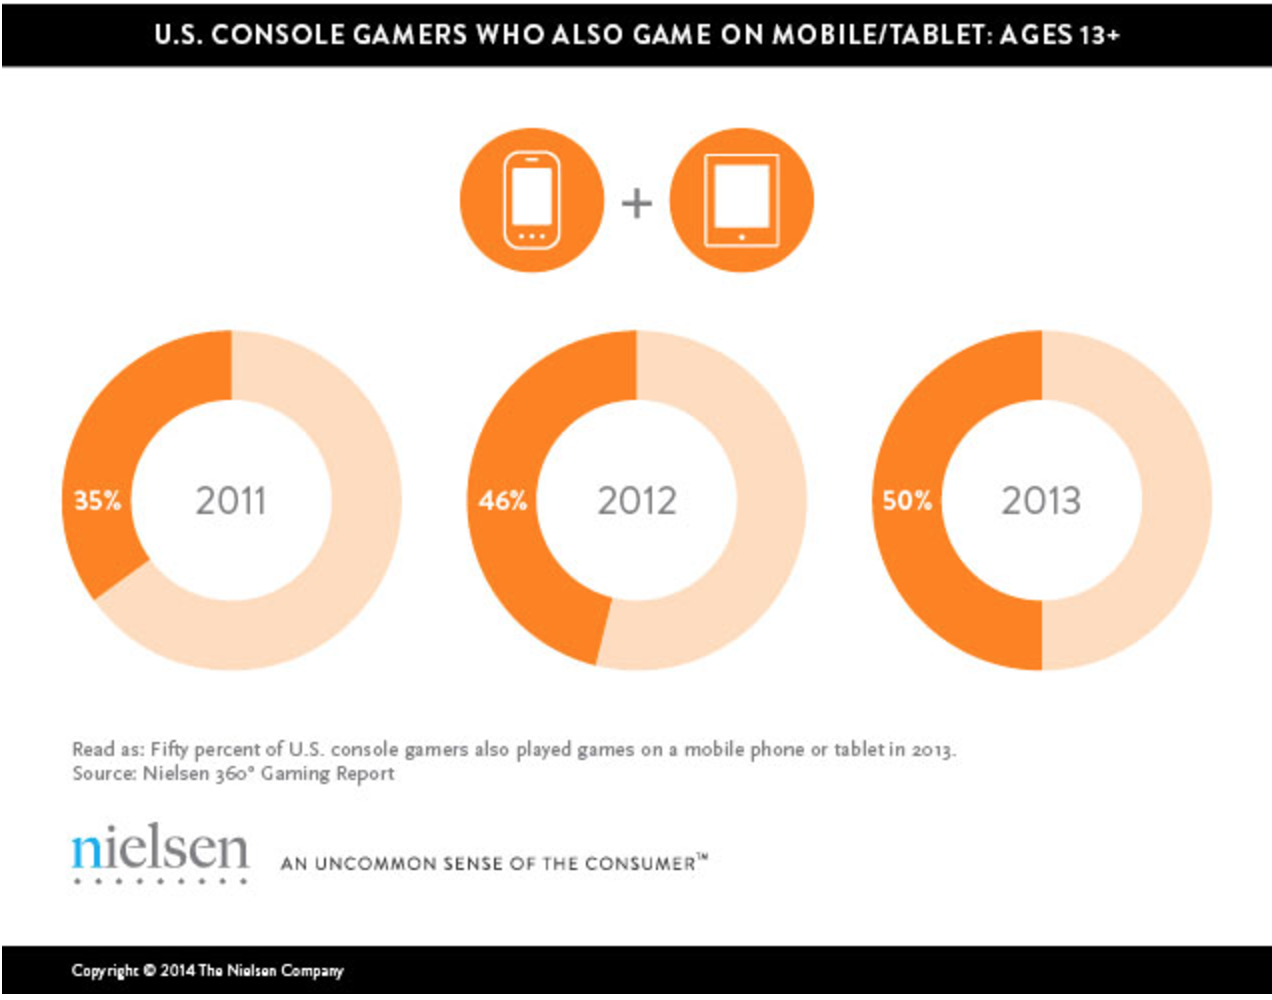
\includegraphics[scale=0.3]{nielsan_tablets_games.png}
    \caption{People are increasing the platforms that they play games on.}
    \label{fig:nielsan_games}
  \end{center}
\end{figure}

According to a study by Nielsen, the number of hours people are spending playing games is increasing.  Users have increased their average game time by an hour a week from 2011 to 2013, which is not terribly surprising.  What is surprising is shown in Figure \ref{fig:nielsan_games}.  Users are starting to play across multiple devices more often.  In 2013, 50 percent of all "gamers" were playing on a mobile device and another device such as their desktop machine or gaming console \cite{nielsan_games}.

Clash of Clans is one of the best examples of a video game that embodies the liquid web framework.  In the game, the user starts with a handful of resources and has to grow their base and army.  The best way to grow is to attack your neighbor, who is another user trying to build their own virtual empire.  So, users take their respective armies and march them onto enemy territory in hopes of concurring new land.  The user plays the role of an army general is responsible for "training" new units and "constructing" new buildings.

This isn't a new concept in gaming.  Real Time Strategy (RTS) games have existed for a long time.  What makes Clash of Clans different is it's use of liquid web concepts.  Clash of Clans can be played from a web browser (mainly on Facebook.com) and on native mobile applications.  In a traditional RTS, the construction of buildings and units takes time typically within minutes.  As you start to expand and construct more advanced buildings and units, the time increases.  With Clash of Clans, some items in the game can take \textit{days} to build.  The user though doesn't need to be logged on during the entirety of that time in order to finish these tasks.  That would be an unrealistic expectation.  Instead, Clash of Clans continues doing the "building" in the background.  Once the time has elapsed, the user has access to the item.

In this example, the user's state changes each time they do an action, or try and build a building or unit.  That state should be reflected across all of their devices, because the user could be one their phone on the train ride home, but then hop onto their laptop as soon as they are back home.  In order for a game like Clash of Clans to work, it has to use the liquid web framework and maintain a user's state on its central server.  Many of the most popular games on mobile devices replicate this model.

There is a distinction here between \textit{saving} a user's content so that it can be accessed from anywhere, and \textit{enabling} the user to seamlessly transition between devices.  While saving the user's state to a server is certainly important, there is nothing new about saving data to a central location and then recovering it on another device.  What's groundbreaking about games like Clash of Clans is that they allow the user to leave mid-action and recover that action on another device.  Even today, most games are tied to the device that they run on, but Clash of Clans and other social network based games show the potential of the liquid web framework in gaming.

\section{Web 3.0 - The Semantic Web}
Web 2.0 was a huge leap in the evolution of the web.  Instead of having a few content publishers and many consumers, the web transformed into a platform where everyone had the ability to publish their content and share their stories.  This also gave rise to the concept of a liquid web where a user's actions and activities should be able to move with them as they transitioned between their devices.  Of course, evolution never stops and so there is now a new shift in the web called \textit{the semantic web} which is also being referred to as Web 3.0.

The semantic web promises direct access to raw data not currently available on the Web or bound up in hypertext documents.  Web 1.0 was the connection of documents via hyperlinks, which enabled users to start in once place and follow related content across the web.  Web 2.0 still relies on this underlying hyperlink structure.  Google's PageRank algorithm ranks pages according to the number of incoming and outgoing links.  Web 3.0 is a shift into \textit{linked data}, which is a framework for publishing content in such a way that it is machine readable \cite{Heath2011}.

Linked data is an effort to use the Web to create links between data from different sources.   This is different from Web 1.0 and Web 2.0 because they relied solely on hyperlinks to connect pages and data together.  One could argue that Web 2.0 connected people in social graphs via social media applications.  These graphs are proprietary though and run against a fixed dataset.  Web 3.0 wants to enable these connections to be accessed in the HTML of a page directly across the entirety of the Web \cite{Heath2011}.  This a much more vast resource than what Web 2.0 offers.

\subsection{Linked Data}
The linked data framework run on top of the same HyperText Markup Language (HTML), Uniform Resource Identifiers (URIs), and the HyperText Transfer Protocol (HTTP) that Web 1.0 and 2.0 utilize but it also introduces a new format called the Resource Description Framework (RDF).  RDF is used to make typed statements that link arbitrary data points in the world together.  This creates a web of \textit{data} rather than a web of \textit{pages} \cite{Heath2011}\cite{archer}\cite{w3c_semantic_web}.

Linked data is trying to link arbitrary data elements together, and this necessitates a structured way to represent those data elements.  The RDF Vocabulary Definition Language (RDFS) and the Web Ontology Language (OWL) provide a basis for structuring this data.  The RDFS and OWL frameworks are not extensions of HTML but instead are extensions of the Extensible Markup Language (XML).  This information can still be contained within HTML, and can still be rendered, but XML is a subset of HTML\cite{heath_global_data}.

As more pages start linking to the \textit{data} in other pages, and not just the pages themselves, the ability to gather data improves. RDF gives other machines the ability to scrape data of these pages in a structured way.  If you wanted to try and do this in Web 2.0, you would have to try and scrape each of these pages based purely on their HTML structure.  It's doable, but unfortunately, everyone develops their web pages differently.  This can be most easily seen when you try and use an auto-citation site such as EasyBib. In EasyBib, a user can provide a link and EasyBib will go out and gather all of the information necessary to create a citation.

However, it does not work every time. For example, consider what happens when EasyBib wants to find the author of a page.  Sometimes, the author is listed directly below the title of the article.  Sometimes it's at the bottom of the article.   Sometimes its formatted as a header, and sometimes it's formatted as a normal paragraph.  The options are rather endless, and so there is no way for EasyBib to check all possibilities.  There may even be possibilities that EasyBib hasn't considered.  RDF and OWL provide a structured way to represent those data elements.  In RDF, you would likely contain the author in an \textit{author} tag.  Then all EasyBib would have to do is search for the \textit{author} tag and pull out the value contained in there.

\begin{figure}[H]
  \begin{center}
    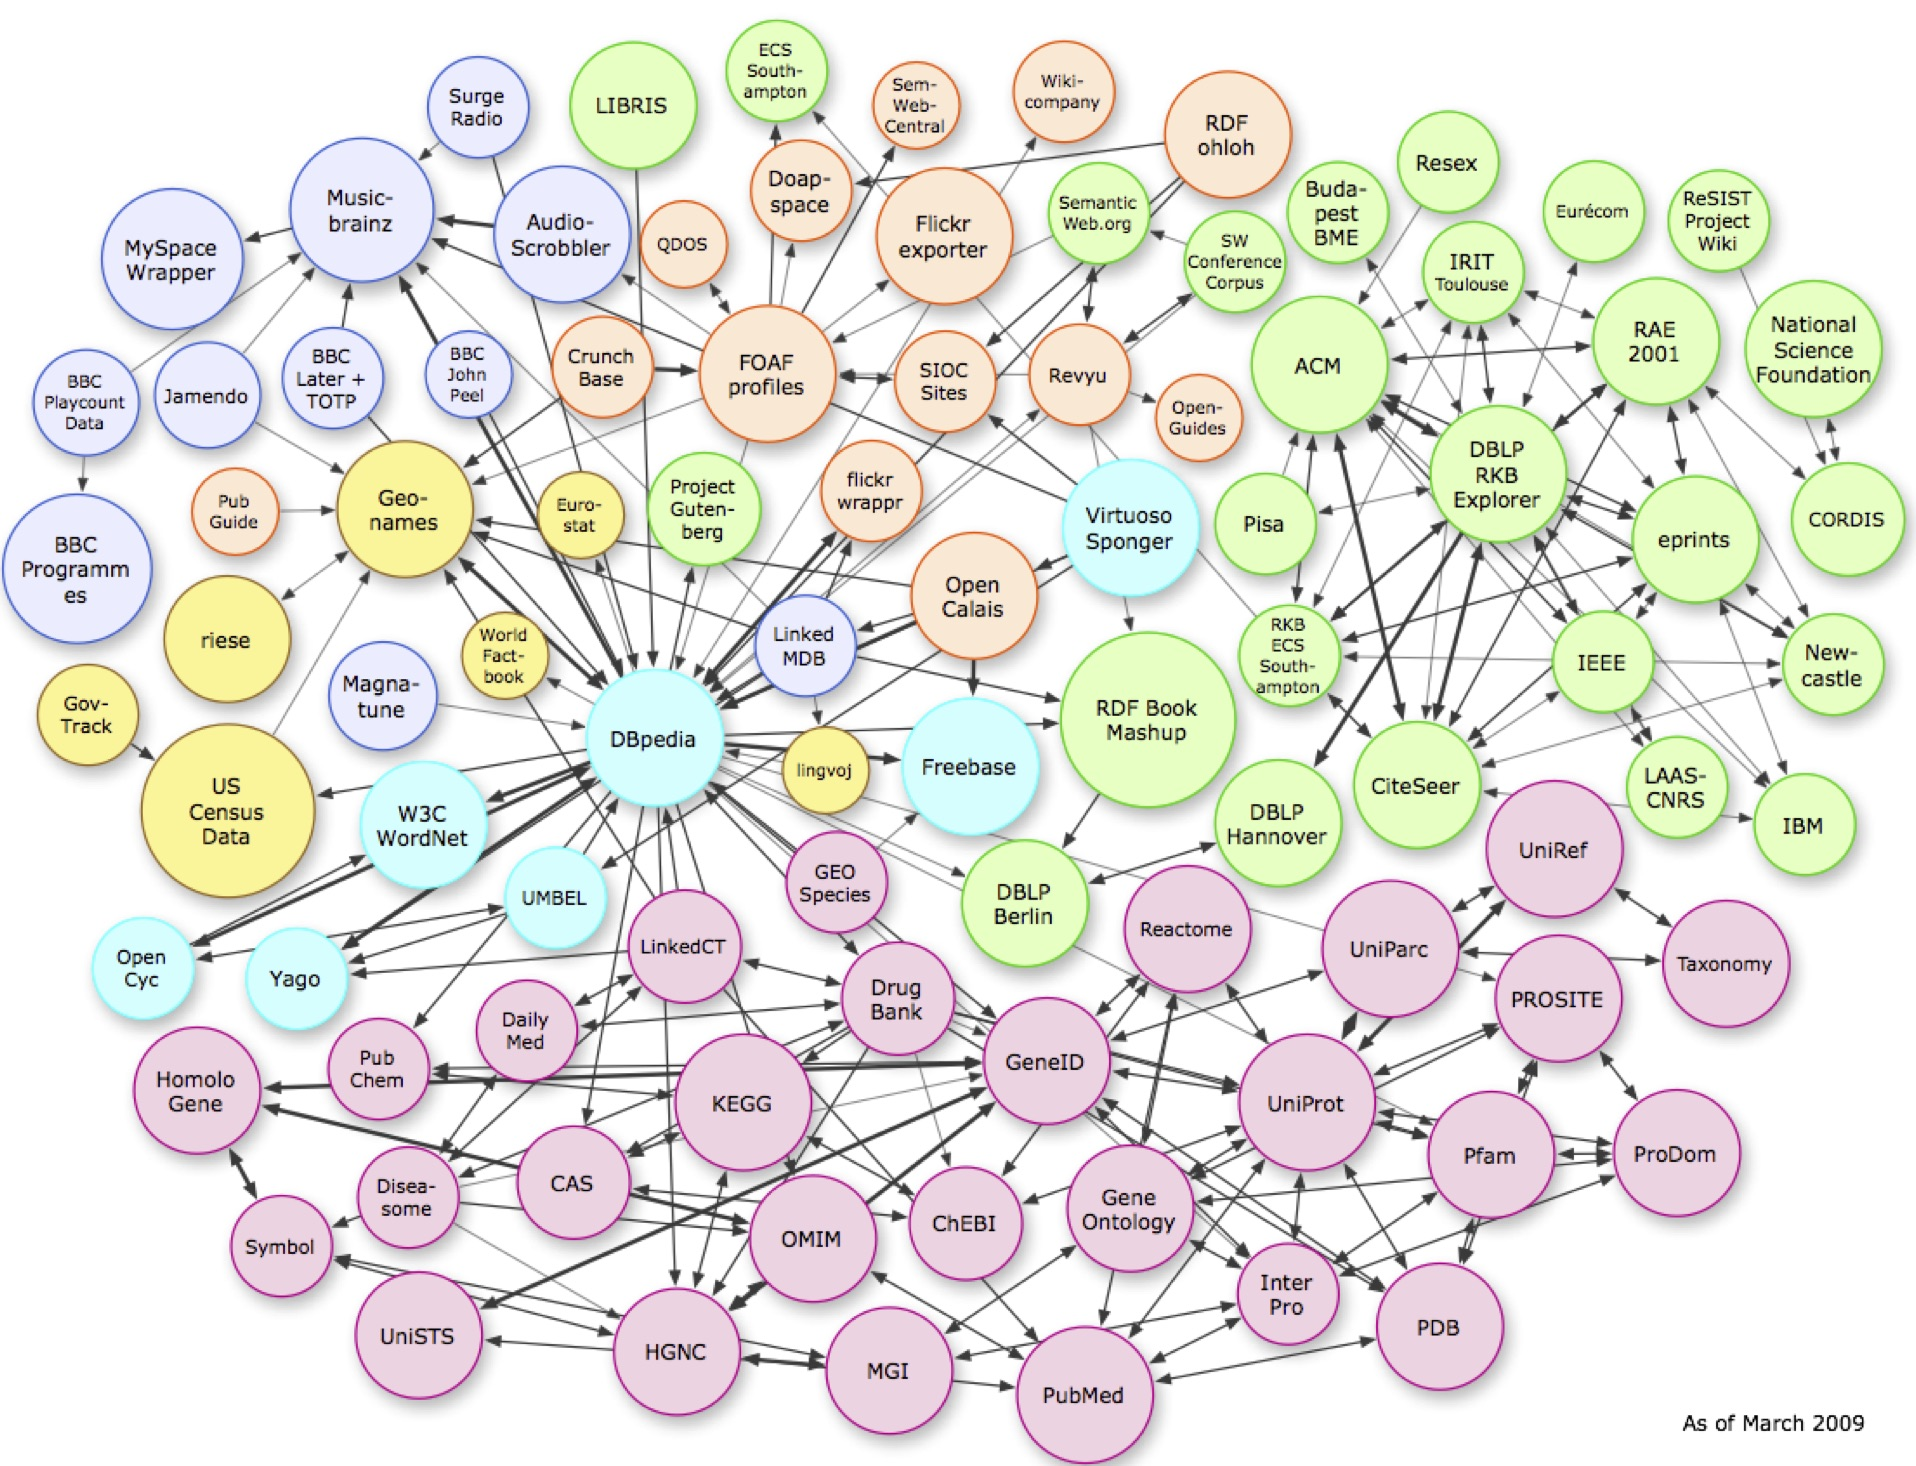
\includegraphics[scale=0.2]{web3_graph.jpg}
    \caption{An example of what a linked data graph looks like.  All of these different pages connect to data in other pages, via RDF, not just hyperlinks.}
    \label{fig:web3_graph}
  \end{center}
\end{figure}

Figure \ref{fig:web3_graph} shows an example of what a linked data graph looks like.  All of these sites are referencing data from another site.  It is similar to how different webpages contain hyperlinks to other pages, and the structure looks similar.  First it is important to note that the graph is directional.  If element \textit{A} has an arrow pointing to element \textit{B}, element \textit{A} references a piece of data with element \textit{B}.  There are still major hubs in the data with lots of incoming and outgoing links.  Again, this is similar to how this works in Web 1.0 and 2.0 with respect to hyperlinks.  In Web 1.0 and 2.0 we would likely consider these sites to be good places to gather information.  If lots of people are referencing a page, it is likely that this page contains the data I want.  The difference here is that these hubs in the linked data framework are actually data hubs.  The information is consumable by another machine and doesn't require a user to make a judgement as to whether or not the data is there.  Machines can also traverse the graph and pull in information into a single resource much faster than a person could.

This process still relies on Web 2.0 principles though.  One of the biggest pillars of Web 2.0 is that the Web becomes stronger the more people that use it. This is especially true in the context of the linked web.  This linking can only happen once  publishers being including the RDF and OWL structured data in their content.  As more people begin to do this, the number of links, and therefore, the richness of the data grows.  Web 3.0 would also enable more data to be immediately available for public consumption.  Web 2.0 made data more available through the use of APIs, but that requires connections and methods for those APIs.  Each API is rather unique, so while Facebook and Twitter may have similar information about a user, the way they represent that information is different.  The Semantic Web, along with Linked Data, aims to remove this inequality.  All of that information is contained within the page and in a structured and well defined way such that the same information can be gleaned from multiple sources.

\section{Conclusion}
The original state of the web create a world in which there were few content publishers, but many content consumers.  In order to access information, users hopped around the web from hyperlink to hyperlink, but this was more than satisfactory for most users.  They still had access to a wealth of information that wasn't available to them previously.  The content consumers though wanted to become the content publishers, and so there needed to be a change in the way that we conceptualized the web.

Web 2.0 was this shift in the industry.  Instead of focusing on a few content publishers with lots of incoming content consumers, Web 2.0 sought to create the "web as a platform" in which anyone could utilize the services that the web provides to create and host their own content.  This change wasn't just centered around content though.  Business models also needed to change.  Google is one of the prime examples of a Web 2.0 business as it wasn't trying to create a native application like Netscape for accessing web content.  Instead they built an application that existed in the Web and was available to anyone with Internet access.

Web 2.0 create a more open and inclusive web.  Companies began opening their proprietary information for open source development, and gave direct access to some of their services via Application Programming Interfaces.  These changes also helped companies leverage the power and ideas of their consumers directly.  One of the major principles of Web 2.0 is that the quality of the Web improves with more collaboration, and now, almost all big companies such as Microsoft, Amazon, and Google all have open APIs that allow developers to collaborate.

This change to a more open and inclusive web, and change in business model to companies that run exclusively on top of the Web also creates a new way of architecting applications.  The Liquid Web is the concept that a user should be able to transition activities and experiences between devices.  When a user starts a task, such as writing an email or viewing a video, on their laptop, they should be able to pick up that task on their mobile phone during their commute.  Users continue to increase the amount of time they spend on mobile devices and it is becoming increasingly important that transitions between devices become seamless.  By using the Web, developers can create Liquid Web applications that achieve this goal.

But Web 2.0 and the Liquid Web are only the beginning.  The "Semantic Web", or Web 3.0, aims to evolve the Web beyond the use of hyperlinks.  While Web 2.0 greatly improves the ability to create and share content, a lot of the value of this content is hidden behind APIs.  A developer could build an application that takes data from Amazon and Twitter using their respective APIs, but each of these APIs has different interfaces and different rules.  The Semantic Web proposes a way of embedding data directly within a site in a standard format such that it is readable and accessible.  Then, developers can leverage data linked across the entire Web and not just contained within individual APIs.  It would greatly improve our ability to enrich applications with data from a variety of sources.

All of these evolutions stem from a continued desire to be more connected to the world around us.  Web 1.0 allowed people to access a wealth of information in an instant.  Web 2.0 then allowed people to contribute directly to this information.  Web 3.0, while not yet fully implemented, will allow us to aggregate this info in a meaningful way and further increase our ability to find the information we want, when we want it.

\clearpage
\bibliography{bibliography}{}
\bibliographystyle{plain}

\end{document}
